
%%%
%%% CHAPTER
%%%
\chapter{Second Law of Thermodynamics}\label{Chapter:FirstLaw}

   \begin{LearningObjectivesBlock}{Learning Objectives}
      Upon completion of this chapter, you will be able to
        \begin{enumerate}
           \item Demonstrate understanding of key concepts of energy and the first law of thermodynamics;
           \item Apply the first law of thermodynamics to assess of heat transfer and power cycles;
           \item Conduct energy analysis of thermodynamic systems;
           \item Employ energy and mass balances into thermodynamic systems to assess efficiency, and correctly observe sign conventions for work and heat transfer.
        \end{enumerate}
\medskip
     Recommended reading: Chapters 5 of \citet{SmithVanNess_Book,Moran_Book,Borgnakke_Book} or 3 of \citet{Atkins_Book}.
   \end{LearningObjectivesBlock}


  
%%%
%%% SECTION
%%%
   \section{Introduction}\label{Chapter:SecondLaw:Section:Intro}
   The first law (Chapters~\ref{Chapter:Introduction} and \ref{Chapter:FirstLaw}) demonstrated that energy can flow either from or to a system in the form of heat or work, however it does not indicate the direction of process (\ie energy flow). The second law of thermodynamics concerns about feasibility, direction and spontaneity of processes and entropy..
   
The second law of thermodynamics is a general principle which makes constraints upon spontaneity of the process, direction of heat transfer and general efficiency of heat engines, \eg a hot body cools to the temperature of the surroundings or a chemical reaction that may run in one direction instead of the reverse (\eg combustion of ethane producing carbon dioxide and water). The reverse of such processes may occur but they will not be spontaneous.  
  
%%%
%%% SECTION
%%%
   \section{Statement of the Second Law}\label{Chapter:SecondLaw:Section:SecondLawStatement}\index{Laws of Thermodynamics ! Second law}
The second law of thermodynamics was stated separately by \citet{Clausius_Book}, Kelvin \citep{Thomson_1851} and \citet{Planck_Book} in slightly different ways. Each statement is based on irreversible processes.
\begin{shaded}
  \begin{center}
    {\bf Clausius Statement}
  \end{center}
  'It is impossible for a self-acting machine working in a cyclic process unaided by any external agency, to convey heat from a body at a lower temperature to a body at a higher temperature.'
\end{shaded}
This statement clearly indicates that heat cannot spontaneously flow from a colder to a hotter body. This can only be realised if other effects play some role, \eg in a refrigeration process in which external work is used to extract heat from low temperature body and reject it into a high temperature body (Fig.~\ref{Chapter:SecondLaw:Fig:SecondLawStatement})

   %%% FIGURE
   \begin{figure}[h]
     \begin{center}
        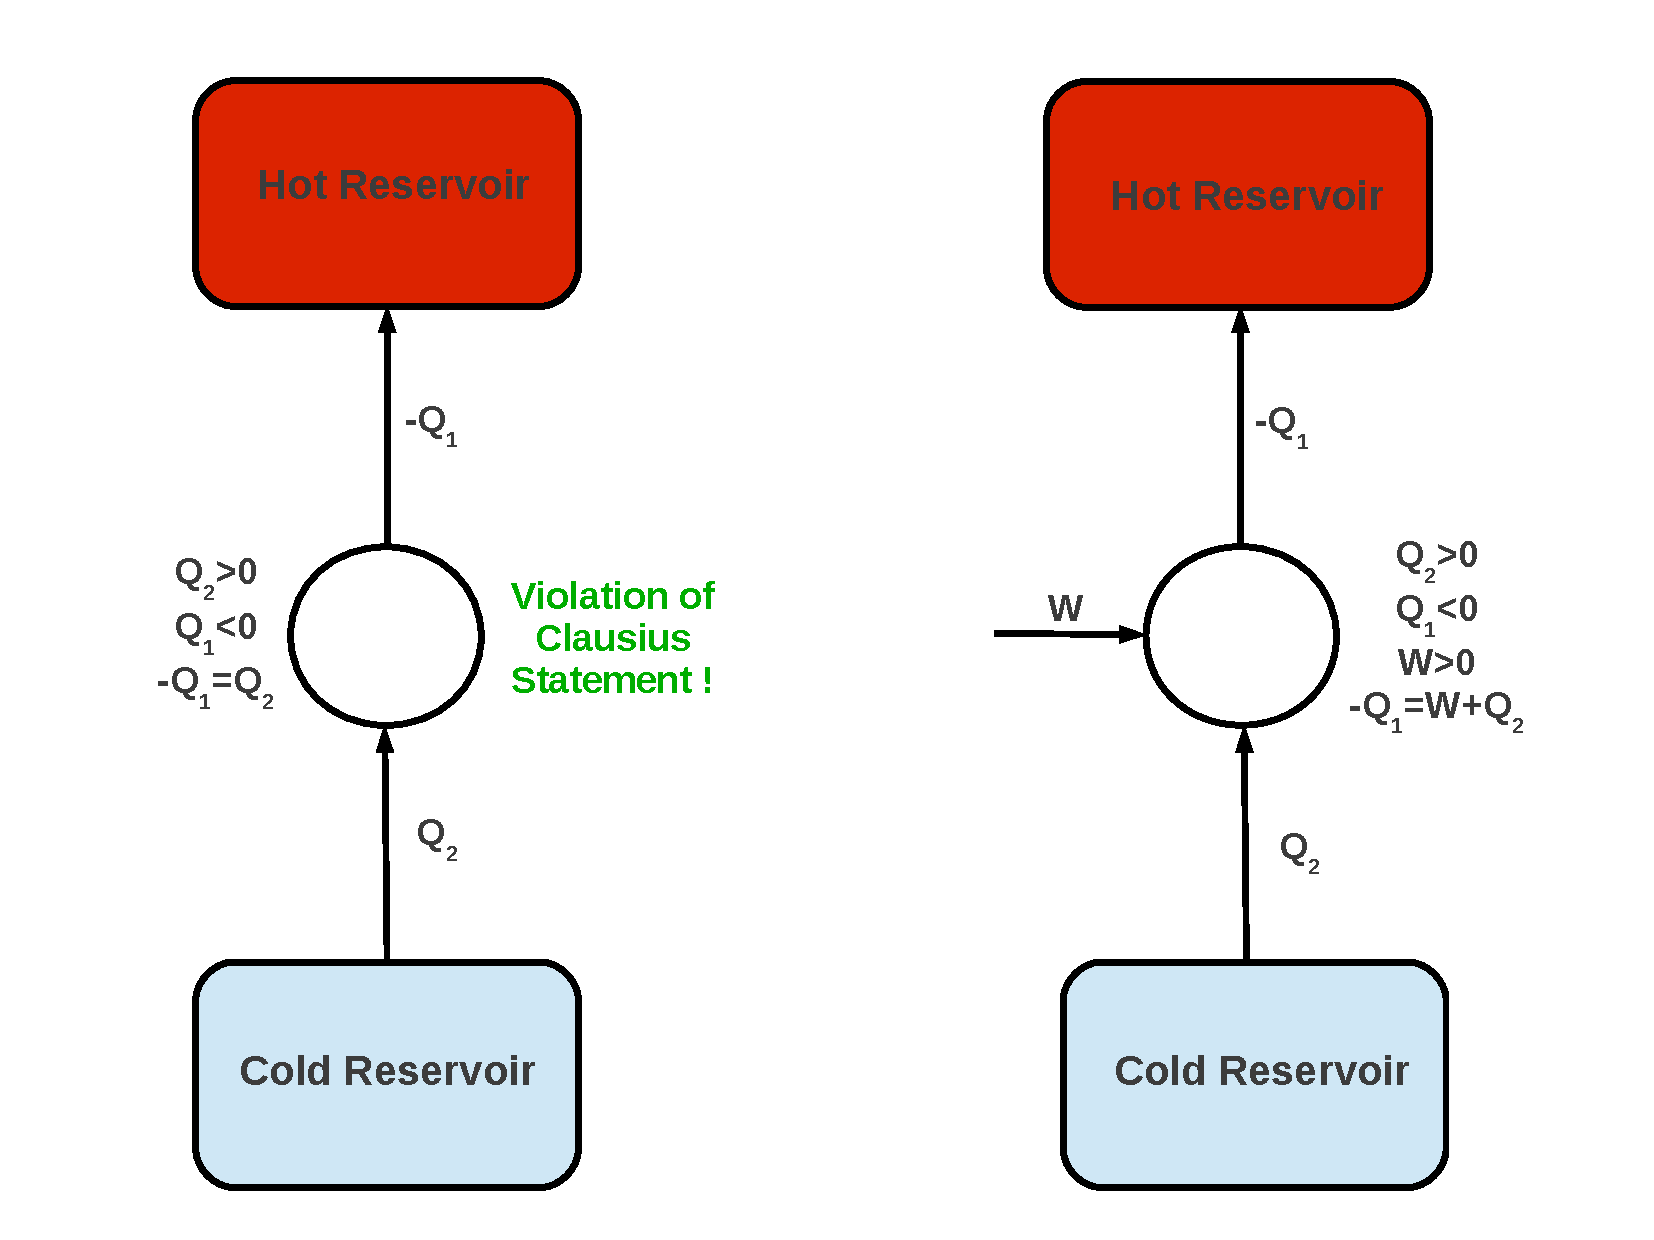
\includegraphics[width=.8\columnwidth,clip]{./Figs/2ndLaw_Schem}
     \caption{All spontaneous processes are irreversible -- heat flows from hot to cold spontaneously and irreversibly. }\label{Chapter:SecondLaw:Fig:SecondLawStatement}
     \end{center}
   \end{figure} 

\begin{shaded}
  \begin{center}
    {\bf Kelvin-Planck Statement}
  \end{center}
  'It is impossible to construct an engine, which while operating in a cycle produces no other effect except to extract heat from a single reservoir and do equivalent amount of work.'
\end{shaded}
This statement indicates that in order to achieve net work from a heat engine (\ie a device operating in cycle), there should be heat interaction between two bodies (\ie thermal reservoirs) at different temperatures (\ie thermal source or sink). 


%%%
%%% SECTION
%%%
   \section{Mathematical Statement of the Second Law}\label{Chapter:SecondLaw:Section:SecondLawStatement_Maths}\index{Laws of Thermodynamics ! Second law}
     \begin{subequations}
        In Fig.~\ref{Chapter:SecondLaw:Fig:SecondLawStatement2}, an infinitesimal amount of heat, $\delta Q^{\prime}$, is transferred from the thermal reservoir (with temperature $T_{res}$) to a reversible cyclic engine (1). The engine produces a small amount of work, $\delta W^{\prime}$, and releases an infinitesimal amount of heat, $\delta Q$ to another reservoir (at variable temperature $T$) that also releases energy in form of work $\left(\delta W\right)$ to the surroundings.

%%% FIGURE
   \begin{figure}[h]
     \begin{center}
        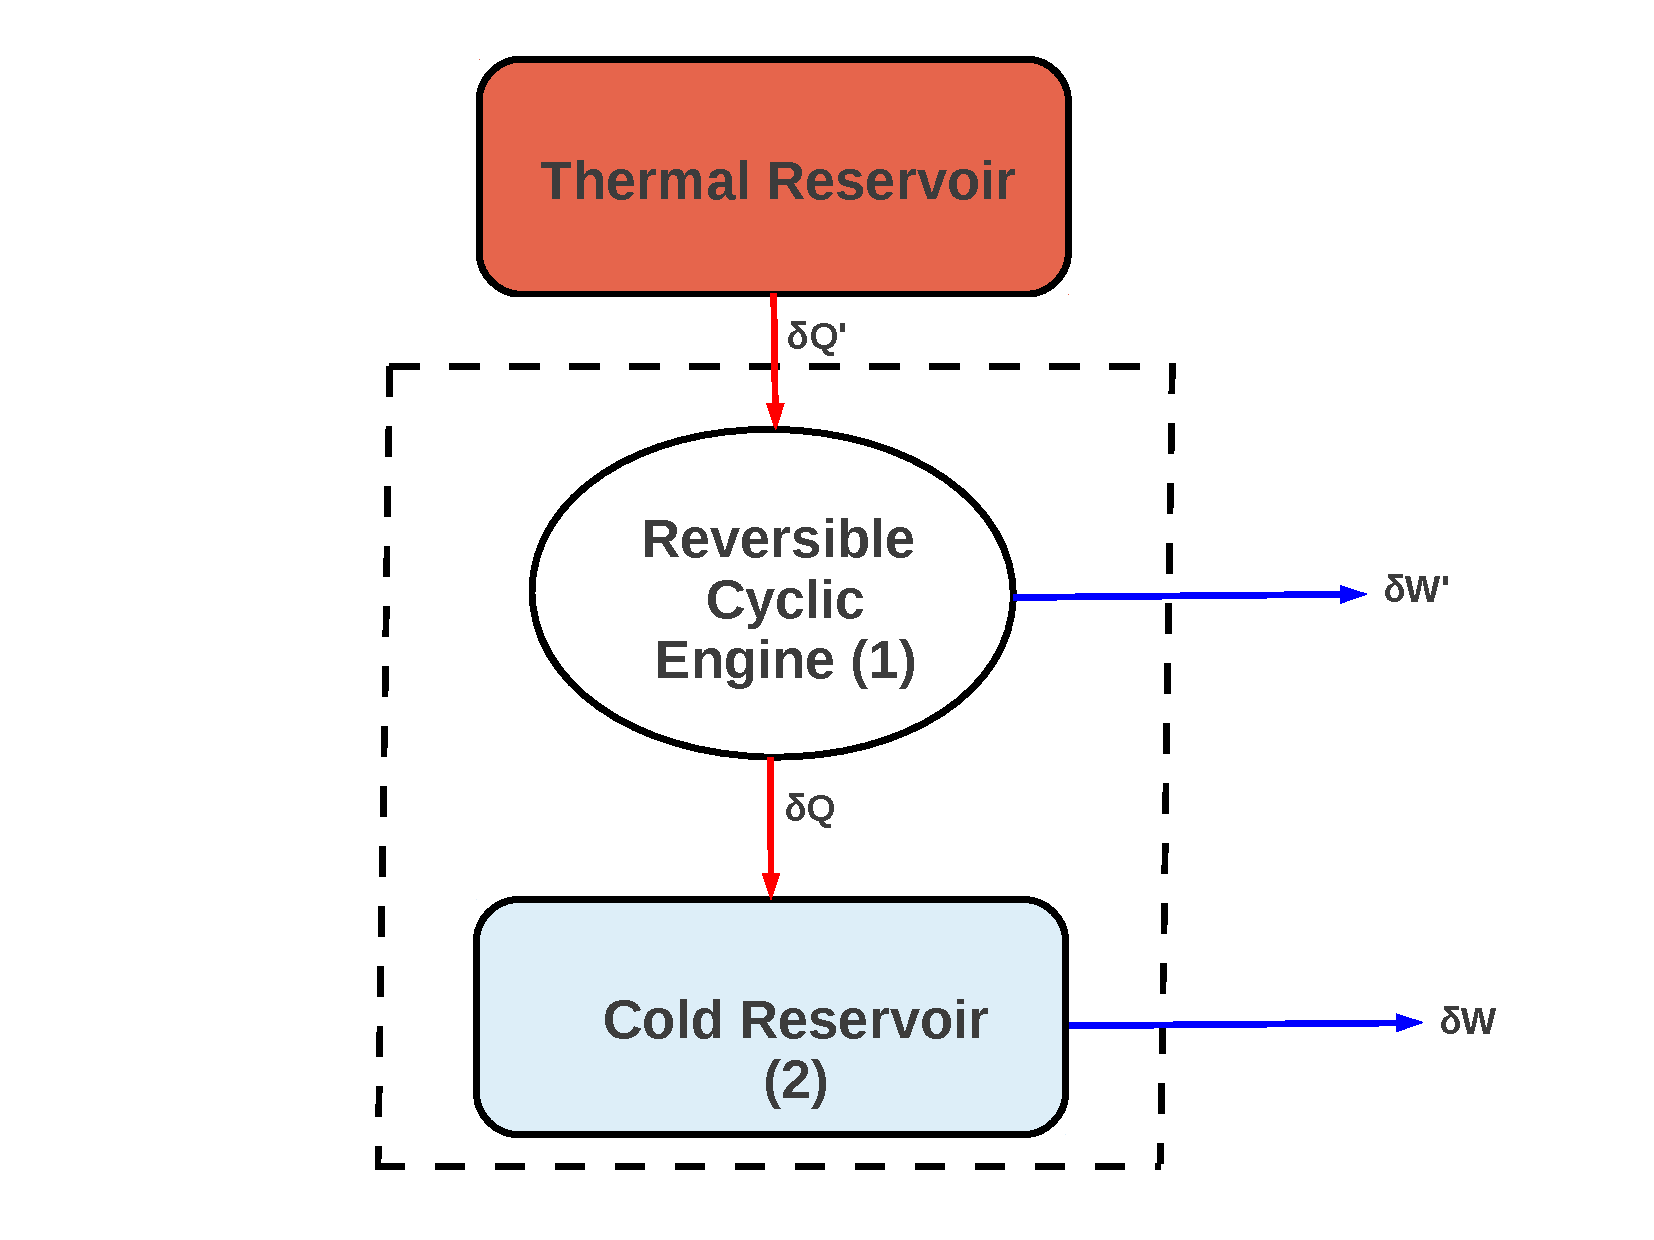
\includegraphics[width=.8\columnwidth,clip]{./Figs/2ndLaw_Schem2}
     \caption{Thermal power device for mathematical derivation of the Second law. }\label{Chapter:SecondLaw:Fig:SecondLawStatement2}
     \end{center}
   \end{figure} 

        Using the analogy of heat transfer ratio and temperature ratio (see power cycle systems in Section~\ref{Chapter:FirstLaw:Section:FirstLaw_Cycle}),
           \begin{displaymath}
              \frc{\delta Q^{\prime}}{\delta Q} = \frc{T_{res}}{T} \;\; \Longrightarrow \frc{\delta Q^{\prime}}{T_{res}} = \frc{\delta Q}{T}.
           \end{displaymath}
        An energy balance (in differential form) for the combined cycle (within the dotted box) is
           \begin{eqnarray}
              && dU = \text{Energy In} - \text{Energy Out} \nonumber \\
              && dU = \delta Q^{\prime} - \left(\delta W + \delta W^{\prime}\right) \Longrightarrow \delta W + \delta W^{\prime} = \delta Q^{\prime} - dU. \nonumber 
           \end{eqnarray}
        Note that the first law is explicitly applied in the second equation above using the sign convention (\ie energy removed from the system is negative whereas energy added to the system is positive). The process is not required to be cyclic and the heat transfer $\delta Q$ is internal and does not cross the boundaries of the combined system. Thus, eliminating $\delta Q^{\prime}$,
           \begin{displaymath}
              \delta W + \delta W^{\prime} = T_{res}\frc{\delta Q}{T} - dU.
           \end{displaymath}
        If the power configuration undergoes a cyclic process,
           \begin{displaymath}
              \oint\delta W + \oint\delta W^{\prime} = \oint T_{res}\frc{\delta Q}{T} -\oint dU,
           \end{displaymath}
        and as $U$ is a thermodynamic property, the cyclic integral is equal to zero.  Integrating the equation above, and assuming that $T_{res}$ is (by definition) constant,
           \begin{displaymath}
              W + W^{\prime} = T_{res}\oint \frc{\delta Q}{T}. 
           \end{displaymath}
        From Kelvin-Planck statement of the Second Law, not all heat can be converted into work, but all work can be converted into heat, thus $W + W^{\prime}\le 0$ (\ie work is always produced in a power cycle and exported to the surroundings) and therefore 

       \begin{shaded}
           \begin{displaymath}
             T_{res}\oint \frc{\delta Q}{T} \le 0.\label{Chapter:SecondLaw:Eqn:SecondLawMathExpression1}
           \end{displaymath}
           Since $T_{res}>0$ (absolute temperature), this integral equation can be divided by $T_{res}$ without changing the meaning of the inequality to obtain the mathematical representation of the Second Law,
           \begin{equation}
             \begin{cases}
                \displaystyle\oint\frc{\delta Q}{T} < 0, & \;\;\text{ for irreversible processes} \\
                \displaystyle\oint\frc{\delta Q}{T} = 0, & \;\;\text{ for reversible processes} 
             \end{cases}\label{Chapter:SecondLaw:Eqn:SecondLawMathExpression2}
           \end{equation}
           This is called {\bf Clausius inequality}.\index{Clausius inequality}
       \end{shaded}
     \end{subequations}

%%%
%%% SECTION
%%%
   \section{Entropy}\label{Chapter:SecondLaw:Section:Entropy}\index{Laws of Thermodynamics ! Second law}
     \begin{subequations}
       Let's consider the reversible process shown in Fig.~\ref{Chapter:Introduction:Fig:CyclesSchematic}, from state 1 to 2, via path {\it A}, and returning to state 2 from either path {\it B} or {\it C}. The Clausius inequality, $\displaystyle\oint\frc{\delta Q}{T} = 0$, can be split as,
           \begin{displaymath}
             \begin{cases}
                \left(\displaystyle\int_{1}^{2}\frc{\delta Q}{T}\right)_{A} + \left(\displaystyle\int_{2}^{1}\frc{\delta Q}{T}\right)_{B} = 0, \\
                \left(\displaystyle\int_{1}^{2}\frc{\delta Q}{T}\right)_{A} + \left(\displaystyle\int_{2}^{1}\frc{\delta Q}{T}\right)_{C} = 0,
             \end{cases}
           \end{displaymath}
       leading to,
           \begin{displaymath}
                \left(\displaystyle\int_{2}^{1}\frc{\delta Q}{T}\right)_{B} = \left(\displaystyle\int_{2}^{1}\frc{\delta Q}{T}\right)_{C} = 0.
           \end{displaymath}
           Since paths {\it B} and {\it C} are different and arbitrary, but $\displaystyle\int\limits_{2}^{1}\displaystyle\frac{\delta Q}{T}$ is the same on either paths -- therefore {\bf the integral is path-independent}. 
           \begin{shaded}
               This defines another thermodynamic property, the {\bf entropy}\index{Entropy},
               \begin{equation}
                  S_{2}-S_{1} = \displaystyle\int_{1}^{2}\frc{\delta Q}{T}.\label{Chapter:SecondLaw:Eqn:Entropy}
               \end{equation}
           \end{shaded}
          Assuming constant mass ($m$), the intensive property entropy $\left(s=S/m\right)$, the differential form is, 
           \begin{displaymath}
                ds = \frc{\delta q}{T} \;\;\;\; \Longrightarrow \;\;\;\; \delta q = Tds,
           \end{displaymath}
           which is the heat transfer equivalent of 
           \begin{displaymath}
                \delta w = \displaystyle\int_{1}^{2}PdV.
           \end{displaymath}
 
           For a reversible process,
           \begin{displaymath}
                S_{2} - S_{1} = \displaystyle\int\limits_{1}^{2}\frc{\delta Q}{T}\;\;\text{ and } \;\; S_{1} - S_{2} = \displaystyle\int\limits_{2}^{1}\frc{\delta Q}{T},
           \end{displaymath}
           and from the Second law
           \begin{displaymath}
                0 \geq \left( \displaystyle\int\limits_{1}^{2}\frc{\delta Q}{T} \right)_{A} + \left( \displaystyle\int\limits_{2}^{1}\frc{\delta Q}{T} \right)_{B}.
           \end{displaymath}
       \begin{shaded}
           These integral expressions can be combined to eliminate path $B$ and obtain a general expression of entropy of arbitrary processes
           \begin{displaymath}
                dS = S_{2}-S_{1} \geq \displaystyle\int\limits_{1}^{2}\frc{\delta Q}{T}
           \end{displaymath}
           where
           \begin{displaymath}
               dS
                \begin{cases}
                      = \frc{dQ}{T} & \;\;\text{ for reversible processes} \\
                      > \frc{dQ}{T} & \;\;\text{ for irreversible processes}.
                \end{cases}
           \end{displaymath}           
       \end{shaded}
     \end{subequations}


%%%
%%% SECTION
%%%
   \section{Entropy Changes}\label{Chapter:SecondLaw:Section:EntropyChanges}
     \begin{subequations}
       From the First Law equation,
           \begin{displaymath}
              dU = dQ - PdV
           \end{displaymath} 
           If we differentiate the enthalpy equation -- $H = U + PV$.
                \begin{displaymath}
                    dH = dU + d(PV) = dU + PdV +VdP,
                \end{displaymath}
           and replace the previous equation,
                \begin{displaymath}
                    dH - \cancel{PdV} - VdP = dQ - \cancel{PdV} \;\;\Rightarrow \;\; dQ = dH - VdP
                \end{displaymath}
           For {\it ideal gas}, $C_{p}=\left(\frac{dH}{dT}\right)_{P}$ and $V=\frc{RT}{P}$,
                \begin{eqnarray}
                  dQ &=& C_{p}dT - \frc{RT}{P}dP\;\;\;\;\;\times\left(\frc{1}{T}\right) \nonumber \\
                  \frc{dQ}{T} &=& \frc{C_{p}}{T}dT - \frc{R}{P}dP \nonumber \\
                  dS &=& \frc{C_{p}}{T}dT - \frc{R}{P}dP, \nonumber
                \end{eqnarray}
           where $S$ is the molar entropy of ideal gas. 
           \begin{shaded}
              Integrating from state 0 to state 1,
                \begin{eqnarray}
                    \int\limits_{S_{0}}^{S_{1}} dS &=& \int\limits_{T_{0}}^{T_{1}} \frc{C_{p}}{T}dT - R\int\limits_{P_{0}}^{P_{1}}\frc{dP}{P} \nonumber \\
                    \left(S_{1}-S_{0}\right) &=& \int\limits_{T_{0}}^{T_{1}} \frc{C_{p}}{T}dT - R\ln{\frc{P_{1}}{P_{0}}} \;\;\;\;\times\left(\frc{1}{R}\right) \nonumber \\
                    \frc{\Delta S}{R} &=& \int\limits_{T_{0}}^{T_{1}} \frc{C_{p}}{R}\frc{dT}{T} - \ln{\frc{P_{1}}{P_{0}}}.\label{Chapter:SecondLaw:Eqn:EntropyChanges1}
                \end{eqnarray}
                Although this equation was derived for mechanically reversible processes, it focuses on \underline{properties only} and is independent of the process. Thus it can be used to calculate entropy changes of {\it ideal gases}. A similar expression can be obtained as a function of $C_{v}$,
                \begin{equation}
                   \frc{\Delta S}{R} = \int\limits_{T_{0}}^{T_{1}} \frc{C_{v}}{R}\frc{dT}{T} +  \ln{\frc{V_{1}}{V_{0}}}
                \end{equation}               
          \end{shaded}
     \end{subequations}
